\chapter{Tesztelés}
A prototípus tesztelése több lépcsőben zajlott: először a hardvert teszteltem, a motorok illesztését, a gearbox működését. Ezután a képfelismerő algoritmusokat hasonlítottam össze, először csak egy statikus kamerával. Mikor elkészültek a 3D nyomtatott alkatrészek, ki tudtam próbálni a kamera célfelismerést és a motorok mozgásának összehangolt működését. Ezzel együtt ki tudtam próbálni, mennyire lett stabil a mechanikai konstrukció, illetve megbízható-e a tüzelés folyamata.

\section{Elektronikai alkatrészek tesztje}
Először csak csatlakoztattam a kamerát a Raspberry Pi megfelelő csatlakozójához, a szalagkábellel, a kamerákat pedig a stepper motor HAT csatlakozóihoz. Ezután a GPIO tüskesorhoz csatlakoztattam a lézer diódát, a relé megfelelő lábait, és a végálláskapcsolókat. A teszt összeállítása a \ref{fig:teszt_1}. ábrán látható.

\begin{figure}
	\centering
	\includegraphics[width=0.6\linewidth]{teszt_1}
	\caption{Elektronikai alkatrészek teszt összeállítása}
	\label{fig:teszt_1}
\end{figure}

A teszt során azt próbáltam ki először, hogy tudom-e mozgatni a motort, működik-e a kamera, a lézer modul, tudok-e lőni a gearboxszal. Minden sikeres volt, így ezt a tesztet lezártam.

\section{Képfelismerő algoritmusok tesztje tesztje}
A teszt összeállítása itt is ugyanaz volt, mint az előző bekezdésben, annyi különbséggel, hogy a kamerát felerősítettem egy állványra, és egy kinyomtatott arcot mozgattam előtte. A célpont a \ref{fig:teszt_facetarget}. ábrán látható. A minta részletei nagyon kontrasztosak, elütnek egymástól, ezzel könnyítve az algoritmusok munkáját.

\begin{figure}
	\centering
	\includegraphics[width=0.6\linewidth]{orctarget2}
	\caption{Az arcfelismeréshez használt kép}
	\label{fig:teszt_facetarget}
\end{figure}

Először két olyan módszert vizsgáltam, ahol a célpont nem általános, hanem egy PNG képet vesz mintának, és ezt keresi a kamera által szolgáltatott képen.

\subsection*{Template Matching}
Erről a módszerről korábban a \ref{sec:soft_template}. bekezdésben írtam. A \code{cv2.matchTemplate()} függvény létrehozza megkeresi a képen sablont, a \code{cv2.minMaxLoc()} pedig visszaadja a helyzetét, valamint az eredmény pontosságát. Az eredmény pontosságának megszabtam egy alsó határt, és azt változtattam a teszt során. Azt tapasztaltam, hogy ez  a módszer nagyon érzékeny a célpont dőlésére és elfordulására, valamint a távolságára is. Semmiképpen nem optimális a feladat elvégzésére.

\subsection*{Feature Matching és Target Tracking}
A feature matching elviekben jól kezeli a célpont torzulását, ezért ezzel kísérleteztem a későbbiekben. Az elképzelés az volt, hogy a feature matching megtalálja megbízhatóan a célpontot, majd a target tracking képes lesz gyorsan követni. Amennyiben egyszer megtalálta az algoritmus a célpontot, onnan tényleg pontosan tudta követni, azonban magával a felismeréssel voltak itt is a problémák. Nagyon megbízhatatlan volt, ha az érzékenységet lentebb állítottam, akkor fals pozitívot is mutatott, ha fentebb, akkor pedig nem találta meg a célpontot. A target tracking is csak akkor működött, ha a kamera egy helyben maradt. Ha már a motorok is mozogtak, akkor könnyedén elvesztette a célpontot.

\subsection{Haar Cascade}
Az utolsó módszer, amit teszteltem, az a Haar Cascade és tanított neurális hálók használata volt. Ez az előzőekhez képest meglepően megbízható volt, a célpontot felismerte viszonylag távolról is, akár rossz fényviszonyok között is. A célpont kb 15 fokos dőlése esetén szintén felismerte azt, amit én megfelelőnek találtam. Ezzel a módszerrel folytattam a munkát.



\section{Éles teszt}
A tesztet egy jól megvilágított tanteremben végeztem. Az eszköz egy stabil padon állt, a célpont pedig 5 méterrel előtte, és kb. fél méterrel fölötte. A célpont a \ref{fig:teszt_lolap}. ábrán látható.

\begin{figure}[h!]
	\centering
	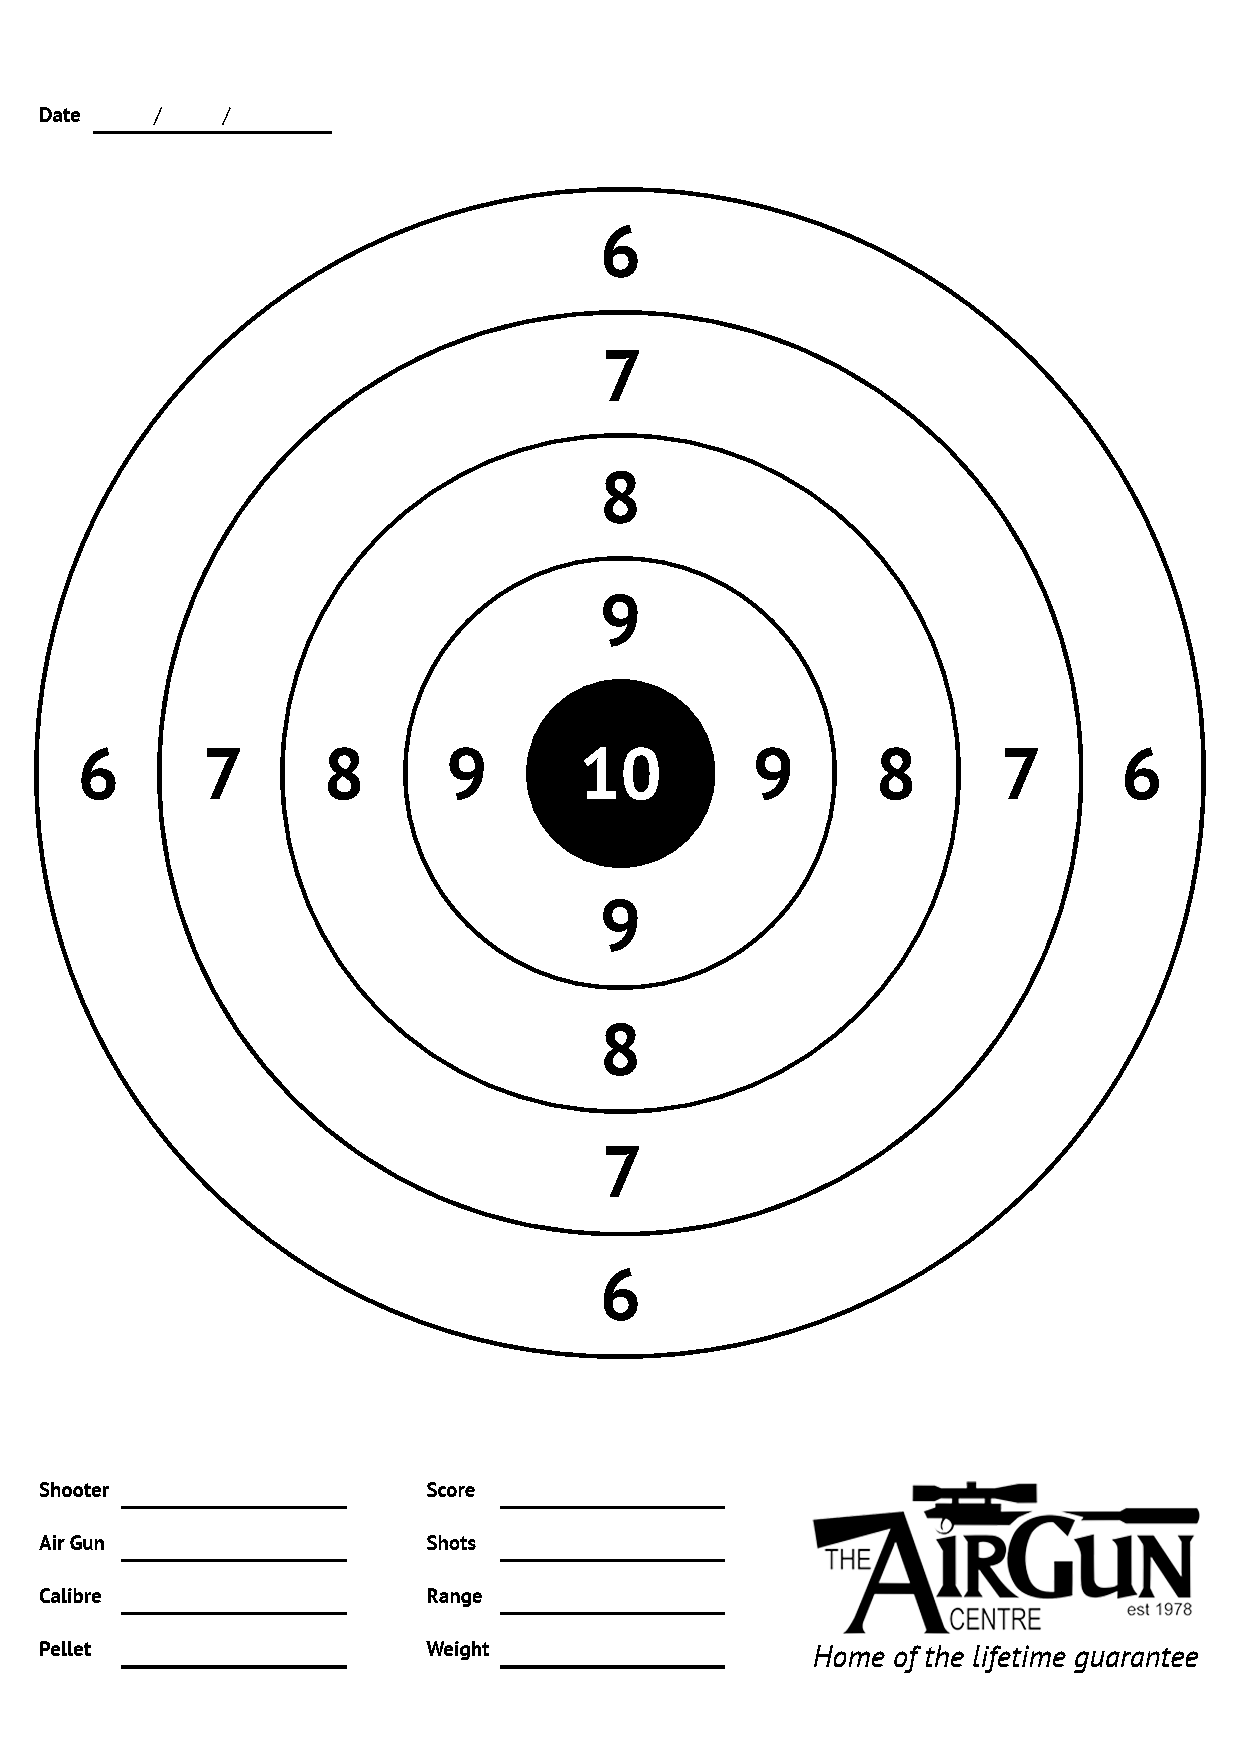
\includegraphics[width=0.4\linewidth]{lolap}
	\caption{Az éles teszthez használt lőlap}
	\label{fig:teszt_lolap}
\end{figure}


A teszt során a manuális működési móddal kezdtem, tulajdonképpen belőttem a fegyvert. Először azt tapasztaltam, hogy a kamera képének a közepe nem ott van, ahova a fegyver csöve mutat. Ezért a célkeresztet addig kellett mozgatnom a képen, amíg oda nem mutatott, ahova a fegyver ténylegesen lőtt. Ezután azt tapasztaltam, hogy nagy pontossággal képes lőni, igen kis területen belül. A lézer irányzékot azonban nem tudtam pontosan beállítani, 5 méteren nagyjából 10-15 cm-t téved. A következő ábrákon látható a teszt eredménye. 5-ös sorozatokban tüzeltem, mindig a cél közepére irányítva a kamera célkeresztjét. \\

A következő teszt az arcfelismerés, és a követés funkció tesztje volt. A körülmények ugyanazok maradtak, és szintén 5 m-re volt a célpont. A teszt során egy kolléga tartotta a kinyomtatott arcképet, és mozgatta, változtatva a sebességet és irányt. Természetesen a gearbox nem volt áram alatt, és a kolléga is viselt védőszemüveget. Azt tapasztaltam, hogy a fegyver körülbelül a sétáló ember sebességét tudja követni 5 m távolságban, és igen pontosan be tudja célozni.


A tesztkörnyezet a \ref{fig:teszt_teszt_setup1}. és \ref{fig:teszt_teszt_setup2}. ábrákon látható.

\begin{figure}
	\centering
	\includegraphics[width=0.6\linewidth]{teszt_setup2}
	\caption{Az éles teszt környezete}
	\label{fig:teszt_teszt_setup1}
\end{figure}

\begin{figure}
	\centering
	\includegraphics[width=0.6\linewidth]{teszt_setup1}
	\caption{Az éles teszt környezete}
	\label{fig:teszt_teszt_setup2}
\end{figure}

Összességében elmondható, hogy a beállított célkereszttel, 5 méterről igen pontos eredmények születtek. 4 leadott sorozat során 5-5 golyót lőttem ki, az eredmények az alábbi ábrán láthatóak:

\begin{figure}[h!]
	\centering
	\includegraphics[width=0.6\linewidth]{teszt_eredmenyek}
	\caption{Az éles teszt eredményei}
	\label{fig:teszt_eredmenyek}
\end{figure}